\documentclass[12pt]{paper}
%\usepackage{paper} %if the document does not compile properly for you on the initial build, uncomment \usepackage{paper} and build again. This should force MikTeX to install package "paper"
\usepackage[margin=1in]{geometry}
\usepackage{float}
\usepackage{natbib}
\bibliographystyle{apsr}
\usepackage{graphicx}
\graphicspath{ {../fig/} }
\usepackage{setspace}
\usepackage[super]{nth}
\usepackage{booktabs}
\usepackage{makecell}
\usepackage{amsmath}
\usepackage{dcolumn}
%\usepackage{authblk}
\usepackage{hyperref}
\usepackage{wrapfig}
\usepackage{amsmath}
%\usepackage{etoolbox}
%
%\AtBeginEnvironment{quote}{\singlespacing\small}
%\usepackage{epigraph}

\begin{document}

\title{Give a Man a Fish and He'll Eat for a Day, But Will He Vote for You?: A Formal Approach to Federal Redistribution and Voter Behavior}
\author{Sarah R. Warren}
\date{\today}
\maketitle
%\epigraph{QUOTE}{\textit{ATTRIBUTION}}
\setstretch{2}
%\thispagestyle{empty}
%\clearpage
%\setstretch{1}

\section{Introduction}
Voter participation is among the most widely studied components of political behavior. Scholars have long considered the individual, social, and systemic factors that influence the decision to show up to the polls on election day. It is well-established and generally accepted that voters with higher education and income turnout more often than their lower-resourced counterparts (Wolfinger and Rosenstone 1980).  Despite its ubiquity, however, few scholars have tried to reconcile the established reality that aid-receiving voters turnout in relatively low numbers with dominant theories of voter behavior.

Seymour Lipset (1960) argued that one's decision to vote depends upon the perceived “relevance of government policies to the individual.” Modern theories of voting behavior—prospective voting (Conover, Feldman, and Knight 1987), retrospective voting (Conover, Feldman, and Knight 1986), sociotropic voting (Hansford and Gomez 2015), and others (Dowding 2005; Fedderson and Sandroni 2006)—still rely on Lipset’s (1960) summation of the boundedly rational political actor: voters turnout based on the perceived relevance of policies to their lives. Thus, what matters is not simply the objective relevance of government to the voter, but the extent to which government agents can effectively claim credit (or avoid blame) for governmental action that citizens perceive to affect them. Presumably, then, those who stand to benefit the most from generous government policies (and, conversely, be most harmed by social spending cuts) should be likely to vote, particularly if they participate in aid programs that assist in feeding their families, provide health insurance, and meet other immediate, tangible needs.

Welfare recipients have an unusually visible stake in elections and policy outcomes. Given such strong personal incentives, one might expect welfare recipients to be more politically active than other citizens (Lipset 1960; Olson 1965); however, this does not appear to be the case in the United States. In fact, public assistance recipients are an especially quiescent voting bloc (Verba, Schlozman, and Brady 1995). 47\% of eligible adults with family incomes of less than \$20,000 a year voted in 2012 and just 25\% voted in the 2010 midterm elections. Additionally, participants in means-tested federal aid programs—those for whom the actions of those in office are most relevant to their day to day lives—are less likely to vote than those who participate in universal, or non-means-tested, aid programs (Mettler and Stonecash 2008).  

As political scientists, how can we reconcile our theoretical predictions with this counterintuitive behavior? I build on existing theories of attribution and voter behavior to model a novel theoretical explanation for the voting behavior of American welfare recipients. I empirically evaluate the implications of my model using data from the Maxwell Poll from 2004-2007. Using a novel measurement technique to classify aid-types, I find that entitlements are associated with an increase in self-reported turnout in elections while government subsidized loans are associated with a decrease in self-reported turnout. Importantly, the effect of means-tested aid on government turnout appears to be less straightforward than previous work suggests.

%[EXPLANATION OF THE FLOW OF THE PAPER – WRITE LAST]%

%\section{The Quiescence of Aid Recipients}
%%revising

\section{A Formal Model of Aid and Attribution}
\emph{Players:} Two politicians, an incumbent (I) and a challenger (C), who have different ideal points $(x_I=1, x_C=0)$. A voter (V) whose ideal point $x_V \epsilon [0,1]$ lies somewhere between $x_I$ and $x_C.$

\emph{Player Types:} Nature selects the politicians’ types, $\theta_I,\theta_C \epsilon {0,1}$, with probabilities: $Pr(\theta_I=0)=Pr(\theta_I=1)=Pr(\theta_C=0)=Pr(\theta_C=1)= \frac{1}{2}$ Nature privately reveals $\theta_I,\theta_C$ to I and C, respectively. Type $\theta=0$ prefers not to deliver aid the voter though delivers aid with some positive probability. Type $\theta=1$ prefers to deliver aid though fails to deliver aid with some positive probability. The probability that the politician delivers aid in accordance with his type is $p > 1 – p$ or $p > \frac{1}{2}$

\emph{Sequence of Play}
\begin{enumerate}
	\item Nature determines each politician’s type, $\theta_I, \theta_C \epsilon {0,1},$ with probabilities $(\frac{1}{2}, \frac{1}{2})$ and reveals types privately to I and C, respectively.
	\item Nature draws from the incumbent’s urn to pick the first period aid amount, $y_1\epsilon {0,1}.$ The incumbent responds according to his type with greater likelihood than not. First period aid $y_1\epsilon {0,1}$ is administered.
	\item Nature determines the cost of voting, $c~U[0,1]$ and reveals this cost to voter V.
	\item The voter V chooses whether to vote, $v\epsilon{0,1}$
	\item If V votes $(v=1)$, then he decides the election winner, I or C. If V does not vote $(v=0)$, Nature decides the election winner, I or C.
	\item The winner (I or C) picks the second period aid amount, $y_2\epsilon {0,1}$. The winner responds according to his type with greater likelihood than not. Second period aid  $y_2 \epsilon {0,1}$ is administered.
\end{enumerate}

\emph{Politicians' Utility}: In each period $t\epsilon{1,2}$, each politician $p\epsilon{I,C}$ receives: 

$U_{p}^t = -|\theta_p - y_t|$

where $y_t\epsilon {0,1}$ is the executive’s choice of distributive aid policy. $\theta_p$ denotes the politician’s type, which represents her preferred distributive policy. Hence, a politician of type $\theta_p=1$ prefers to deliver aid $(y_t=1)$, while a politician of type $\theta_p=0$ always prefers no aid $(y_t=0).$

\emph{Voter's Utility}: V’s utility function is constant across periods: 

$U_{p}^t = -|x_o - x_V| + y_t$

where $y_t\epsilon{0,1}$ represents the amount of distributive aid awarded to the voter in period $t\epsilon{1,2},$, $x_V$ represents the voter’s ideal point, and $x_o$ is the ideal point of the office-holding politician, who is either the Incumbent $(x_I=1)$ or the Challenger $(x_C=0).$ Hence, the voter’s utility depends on his ideological proximity to the office holder as well as his benefit from any distributive aid.

In between the two periods, the voter may choose to vote in the election by incurring a turnout cost, $c$, which is randomly drawn by Nature from the uniform distribution $c~U[0,1]$ and revealed to $V$ prior to the election. $V$’s payoff for the entire game is therefore given by:

$U_{V}^1 + U_{V}^2 - c \times v$

where $v\epsilon{0,1}$ is V’s choice of whether to turn out in the election, and $U_{V}^1$ and $U_{V}^2$ are V’s payoffs from the first and second periods, respectively.

\emph{Voter Beliefs}: The Voter V does not observe the politician types, $\theta_I$ and $\theta_C$, that Nature randomly chooses. Instead, V can only observe the Incumbent's first-period distributive policy,  $y_1$, and form updated beliefs about I’s type. Let $p_(\theta_I ) (\theta_p | y_1 )$ denote the V’s posterior beliefs about the probability that $\theta_I=1$ after observing $y_1$.

\subsection{Equilibrium Outcomes}
	For simplicity, I assume that Voter V resolves indifference in favor of abstaining.
	
\textbf{Lemma A (Executive’s Distributive Policy):} In each period $t\epsilon{1,2}$, the office-holding executive, $p\epsilon{I,C}$, chooses the distributive policy: 

$x_t=\theta_j (1-p)+ \theta_i (p)$, 

where $\theta_j$ is the opposite of the office holder’s type. Incumbent types are therefore not fully separating. 


\textbf{Lemma B (Voter’s updated beliefs about Incumbent’s type):}  After observing the Incumbent’s choice of $y_1 \epsilon {0,1}$ during the first period, the Voter V’s updated belief about the Incumbent’s type is: $p_(\theta I) (p(\theta_i ) + (1 - p)(\theta_j ) | y_1 )=y_1$.

Given Lemma B, V expects to receive $E(y_2 | e=I)=p(\theta_i )+(1-p)(\theta_j)$ units of aid in $t=2$ if I is reelected and $E(y_2 |e=C)=E(\theta_C )=\frac{1}{2}$ units of aid if C wins the election.  V’s expected second period payoff from I’s reelection would be: $EU_V (e=I) = -(1 - x_v ) + [p(y_1 ) + (1 - p)(y_1 )]$ whereas his expected second period payoff from C’s election would be: $EU_V (e=C) = - x_V + \frac{1}{2}$. Therefore, conditional on turning out, V votes for I iff: 

$EU_V (e=I) \geq EU_V (e=C) \Rightarrow = -(1 - x_V ) + [p(y_1 ) + (1 - p)(y_1 )] \geq - x_V + \frac{1}{2} \Rightarrow x_V \geq \frac{3}{4} + \frac{p(y_1 - y_-1 ) + y_-1}{2}$

When $x_V$ is above this threshold, V prefers that the Incumbent win the election, so V’s total expected payoff from voting would be:
$ EU_V (v=1 | x_V \geq \frac{3}{4} + \frac{p(y_1 - y_-1 ) + y_-1}{2}) = - (1 - x_V ) + y_1 - c$

When $x_V$ is below the threshold, V prefers that the Challenger win the election, so V’s total expected payoff from voting would be:
$ EU_V (v=1 | x_V \geq \frac{3}{4} + \frac{p(y_1 - y_-1 ) + y_-1}{2}) = -x_V + \frac{1}{2} - c$

In both cases, V’s total combined expected payoff from not voting is:
$ EU_V (v=0) = \frac{EU_V (e=I)}{2} + \frac{EU_V (e=C)}{2} + \frac{- (1 - x_V ) + y_1}{2} + \frac{-x_V + \frac{1}{2}}{2} = \frac{y_1}{2} - \frac{1}{4}$

Hence, in equilibrium, V turns out to vote iff: $EU_V (v=1) \geq EU_V (v=0) \Rightarrow c \leq \bar{c}$ where:

\begin{equation}
\bar{c} =
\begin{cases}
\frac{-y_1}{2} - x_V + \frac{3}{4} & if x_V < \frac{1}{4}\\    
x_V (2y_1 - 1) + \frac{3}{4}     & if \frac{1}{4} \leq x_V < \frac{3}{4}  \\
\frac{y_1}{2} + x_V - \frac{3}{4}     & if x_V \geq \frac{3}{4}  \\
\end{cases}
\end{equation}

\textbf{Lemma C: (V’s Turnout and Vote Choice):} Let $Q_(y_1 )(x_V )$ denote the probability of turnout for a voter with ideal point $x_V$ and who receives $y_1 \epsilon {0,1}$ of aid during Period 1. V’s turnout choice in the election is:

\begin{equation}
Q_(y_1 )(x_V ) =
\begin{cases}
\frac{-y_1}{2} - x_V + \frac{3}{4} & if x_V < \frac{1}{4}\\    
x_V (2y_1 - 1) + \frac{3}{4}     & if \frac{1}{4} \leq x_V < \frac{3}{4}  \\
\frac{y_1}{2} + x_V - \frac{3}{4}     & if x_V \geq \frac{3}{4}  \\
\end{cases}
\end{equation}

Therefore, given turning out, V’s vote in the election is:
\begin{equation}
s =
\begin{cases}
I, & if x_V \geq \frac{3}{4} + \frac{p(y_1 - y_-1) + y_-1}{2} \\    
C,     & otherwise  \\
\end{cases}
\end{equation}
where $y_-1$ is the aid amount not delivered in the period (i.e. if $1$ unit of aid was delivered, $y_-1 = 0$.)

Given this, we can calculate the \emph{change in turnout probability} from receiving one unit of aid in $t_1$. Put differently, the effect of receiving $y_1 = 1$ is:
\begin{equation}
Q_1 (x_V ) - Q_0 (x_V )=
\begin{cases}
\frac{-1}{2} & if x_V < \frac{1}{4}\\    
2x_V - 1 & if \frac{1}{4} \leq x_V < \frac{3}{4}  \\
\frac{1}{2} & if x_V \geq \frac{3}{4}  \\
\end{cases}
\end{equation}

In other words, delivering aid to ideologically distant voters $(x_V < \frac{1}{2})$ strictly decreases their probability of turning out, while delivering aid to ideologically proximate voters $(x_V > \frac{1}{2})$  strictly increases their probability of turning out. Additionally, conditional upon turnout, delivering aid strictly increases the likelihood of voting for the incumbent. The delivery of aid during period one increases V’s expected payoff from having the incumbent reelected relative to the probability that the aid distribution was an informative signal. The increased expected payoff drives my main prediction that the delivery of aid in period one increases a right-wing voter's probability of turnout.

\begin{figure}
	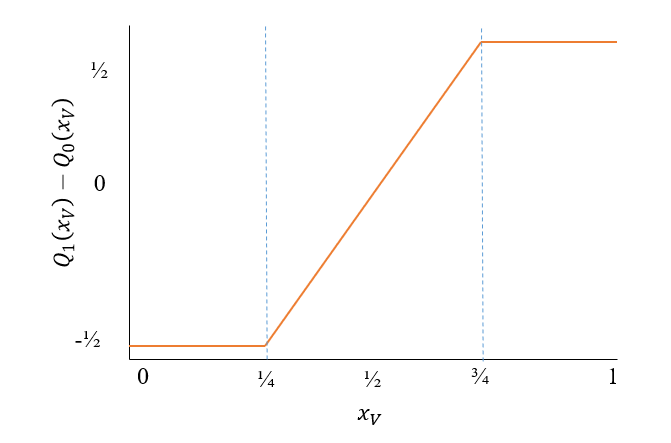
\includegraphics[width=\linewidth]{Figs/equilibrium.png}
	\caption{Figure 1: Change in Turnout Probability Given Aid}
	\label{Figure 1: Change in Turnout Probability Given Aid}
\end{figure}

From Lemmas A, B, and C, we can derive the simple prediction that those who favor the incumbent \emph{a priori} credit the Incumbent with the positive experience of aid and, therefore, turnout to vote for him or her. Those who do not favor the incumbent \emph{a priori}, rather than change their vote choice, are simply less motivated to turnout to oust the Incumbent. Distant voters, therefore, should be less likely to turnout to vote at all. Put differently, receiving aid in $t_1$ causes a relatively larger increase in a right-wing voter’s turnout probability but a relatively smaller decrease in a left-wing voter’s turnout probability, given $p > \frac{1}{2}$. 

\emph{H1(a): For a left-wing voter $(x_V < \frac{1}{2})$, receiving distributive aid in period 1 causes a strict decrease in the probability of voter turnout.\\
H1(b): For a right-wing voter $(x_V > \frac{1}{2})$, receiving distributive aid in period 1 causes a strict increase in the probability of voter turnout.}

%\section{Research Design}
%\section{Analysis}
%\section{Discussion}
%\section{Conclusion}


\end{document}